\documentclass[10 pt,usenames,dvipsnames, oneside]{article}
\usepackage{../../../modelo-ensino-medio}



\begin{document}

\begin{center}
  \begin{minipage}[l]{3cm}

\includegraphics[width=2cm]{logo}    
\end{minipage}\hfill
\begin{minipage}[r]{.8\textwidth}
 {\Large \scshape Atividade: Afim e Exponencial}  
\end{minipage}
\end{center}
\vspace{.2cm}

\ifdefined\prof
%Habilidades da BNCC
\begin{objetivos}
\item \textbf{EM13MAT304} Resolver e elaborar problemas com funções exponenciais nos quais é necessário compreender e interpretar a variação das grandezas envolvidas, em contextos como o da Matemática Financeira e o do crescimento de seres vivos microscópicos, entre outros. 
\end{objetivos}

%Caixa do Para o Professor
\begin{goals}
%Objetivos específicos
\begin{enumerate}
\item Investigar por meio de gráficos as variações da função exponencial em intervalos de tamanho fixo, comparando com a variações da função afim.

\item Identificar os papéis das constantes na expressão da função exponencial $f(x)=ca^{\frac xk}$.
\end{enumerate}

\tcblower

%Orientações e sugestões
\begin{itemize}
\item Após a discussão peça para os estudantes proporem desafios para os colegas: eles mostram $3$ pontos e os colegas tentam “adivinhar” o próximo e fornecer a expressão analítica.
\end{itemize}
\end{goals}

\bigskip
\begin{center}
{\large \scshape Atividade}
\end{center}
\fi

\begin{enumerate}
\item{} O gráfico (A) representa a função afim $y=3+\dfrac{1}{4}x$. Explique como os números $3$, $1$ e $4$ que aparecem na expressão da função afetam ou “aparecem” no gráfico.

\item{} O gráfico (B) representa o crescimento exponencial dado pela expressão $y=1 \cdot 3^{x/4}$. Explique como os números $3$, $1$ e $4$ que aparecem na expressão da função afetam ou “aparecem” no gráfico.

\item{} Os três pontos representados abaixo pertencem a uma curva de crescimento exponencial. Determine o ponto de abscissa $x=15$ que mantém esse crescimento e escreva uma expressão que descreva a curva.

\begin{figure}[H]
\centering
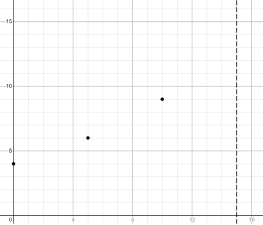
\includegraphics[width=200bp]{pontos.png}
\end{figure}
\end{enumerate}

\ifdefined\prof
\begin{solucao}

\begin{enumerate}
\item $3$ é o intercepto-y, $1$ é o deslocamento vertical que corresponde a um deslocamento horizontal de $4$ unidades.

\item
$1$ é o intercepto-y (valor inicial), a cada $4$ unidades de deslocamento horizontal o valor anterior fica multiplicado por $3$.

\item
Valor inicial $4$ e a cada $5$ unidades de deslocamento horizontal, multiplicamos por $\frac 64=\frac 32$. Assim, para $x=15$ teremos $f(15)=9\cdot \frac 32=13{,}5$.
A expressão então é dada por $f(x)=4\cdot \left(\dfrac 32\right)^{\frac x5}$.
\end{enumerate}

\end{solucao}
\fi

\end{document}